\documentclass[a4paper]{article}
\usepackage{url} 
\usepackage{geometry}
\usepackage{graphicx}
\usepackage[parfill]{parskip}
\usepackage{pgfplots}
\usepackage{pgfplotstable}
\pgfplotsset{compat=newest}
\usepgfplotslibrary{fillbetween}

\definecolor{printred}{RGB}{215,25,28}
\definecolor{printorange}{RGB}{253,174,97}
\definecolor{printyellow}{RGB}{255,255,191}
\definecolor{printgreen}{RGB}{145,180,130}
\definecolor{printblue}{RGB}{43,131,186}
\definecolor{printlilac}{RGB}{178,171,210}

\begin{document}
\begin{figure}[ht]
\pgfplotstableread[col sep=comma]{data/pstate_power_4_cores.csv}\pstatelavamdtable
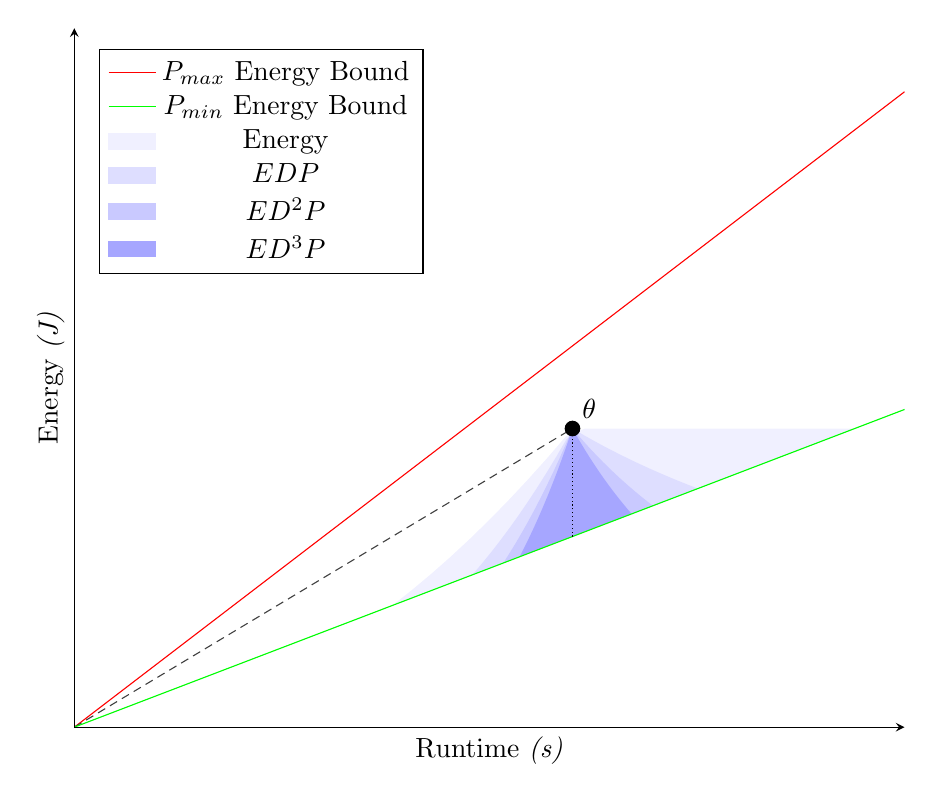
\begin{tikzpicture}
  \begin{axis}[ticks = none, 
    axis on top,
    axis x line=bottom,
    axis y line=left,
  	xlabel={Runtime \emph{(s)}},
    ylabel={Energy \emph{(J)}},    
    xmin=0, xmax=50,
    ymin=0, ymax=3300,
    width=\linewidth,
    legend style={legend pos=north west}
    ]

    %% Model Parameters %%
    \pgfmathsetmacro{\baselinepower}{30} % NOP code
    \pgfmathsetmacro{\rooflinepower}{60}
    \pgfmathsetmacro{\codepower}{47} 
    \pgfmathsetmacro{\codetime}{30}

    %% Intermezzo Values %%
    \pgfmathsetmacro{\codeenergy}{\codepower * \codetime}
    \pgfmathsetmacro{\baselineenergy}{\baselinepower * \codetime}
    \pgfmathsetmacro{\rooflineenergy}{\rooflinepower * \codetime}

    % arguments: code power, code time, x, n 
    \pgfmathdeclarefunction{metricbound}{4}{%
      \pgfmathparse{((#1 * #2^(#4 + 1)) / #3^#4)}%
    }
    \pgfmathdeclarefunction{definitionbound}{4}{%
      \pgfmathparse{((#1 / #2^(#4 + 1)) * #3^(#4 + 2))}%
    }
 
    % BETA ROOFLINE BOUND
    \addplot[color=red, domain=\pgfkeysvalueof{/pgfplots/xmin}:\pgfkeysvalueof{/pgfplots/xmax}] {\rooflinepower * x};
    \addlegendentry{$P_{max}$ Energy Bound}

    %const power diagonal
    \addplot[color=darkgray, densely dashed, name path=constpwr, forget plot, %forget plot prevents legend entry
            domain=\pgfkeysvalueof{/pgfplots/xmin}:\codetime] {\codepower * x}; 

    % ALPHA BASELINE BOUND 
    \addplot[color=green, name path=basebound, domain=\pgfkeysvalueof{/pgfplots/xmin}:\pgfkeysvalueof{/pgfplots/xmax}] {\baselinepower * x};
    \addlegendentry{$P_{min}$ Energy Bound} 

    % Constant Time vertical dots
    %vertical
    \draw[densely dotted] ({axis cs:\codetime,\baselineenergy}) -- ({axis cs:\codetime,\codeenergy});

    % Sadly, pgfplots sucks too much to calculate cube roots
    % Domain values are calculated with a ruby script in tools

    %% Energy Area %%
    \addplot[name path=energy, draw=none, domain=19.14894:47, forget plot]{ min(definitionbound(\codepower, \codetime, x, 0),metricbound(\codepower, \codetime, x, 0))};
    \addplot[blue!6] fill between[of=energy and basebound];
    \addlegendentry{Energy}

    %% Energy Delay Product Area %% 
    \addplot[name path=edp, draw=none, domain=23.96806:37.54997, forget plot] { min(definitionbound(\codepower, \codetime, x, 1),metricbound(\codepower, \codetime, x, 1))};
    \addplot[blue!13] fill between[of=edp and basebound];
    \addlegendentry{$EDP$}

    %% Energy Delay Squared Product Area ##
    \addplot[name path=edtwop, draw=none, domain=25.83028:34.84283, forget plot] { min(definitionbound(\codepower, \codetime, x, 2),metricbound(\codepower, \codetime, x, 2))};
    \addplot[blue!21] fill between[of=edtwop and basebound];
    \addlegendentry{$ED^2P$}

    %% Energy Delay Cubed Product Area ##
    \addplot[name path=edthreep, draw=none, domain=26.81496:33.56336, forget plot] { min(definitionbound(\codepower, \codetime, x, 3),metricbound(\codepower, \codetime, x, 3))};
    \addplot[blue!35] fill between[of=edthreep and basebound];
    \addlegendentry{$ED^3P$}




     \node[circle,fill,inner sep=2pt] at (axis cs:\codetime,\codeenergy) {};
    \node[above right] at (axis cs:\codetime,\codeenergy) {$\theta$};
  \end{axis}
\end{tikzpicture}

\end{figure}
\end{document}
